\documentclass{beamer}
\usepackage[utf8]{inputenc}
\usepackage{graphics}
\mode<presentation> {
\usetheme{unc}}
\setbeamertemplate{navigation symbols}{} % To remove the navigation symbols from the bottom of all slides uncomment this line

\usepackage{graphicx} % Allows including images
\usepackage{booktabs} % Allows the use of \toprule, \midrule and \bottomrule in tables


\usepackage{hyperref}
\hypersetup{linkcolor=blue,colorlinks=true}


% Remove symbols
\beamertemplatenavigationsymbolsempty


%\usetheme{default}

\usefonttheme{serif}

%----------------------------------------------------------------------------------------
%	TITLE PAGE
%----------------------------------------------------------------------------------------


\title[Civil Wars 2]{\LARGE{Civil Wars Continued}}
\author[POLI 150]{Steven Saroka}
\institute{POLI 150}
\date{20 February 2024}


\begin{document}

\begin{frame}
\titlepage % Print the title page as the first slide
\end{frame}


%\begin{frame}
%\frametitle{Overview} % Table of contents slide, comment this block out to remove it
%\tableofcontents % Throughout your presentation, if you choose to use \section{} and \subsection{} commands, these will automatically be printed on this slide as an overview of your presentation
%\end{frame}


%----------------------------------------------------------------------------------------
%	PRESENTATION SLIDES
%----------------------------------------------------------------------------------------



	\begin{frame} 
	\frametitle{\LARGE{Announcements}}
	\begin{itemize}
		\item NO CLASS Feb. 22 and 29.
		\item Subject pool module 1 open from Feb. 21 until Mar. 6. Module 2 open from Mar. 27 until Apr. 10. For more information see \href{https://tarheels.live/psspparticipants/}{the PSSP site} or email pssp@unc.edu. Failure to complete the research requirement will result in a grade of IN for the course.
		
	\end{itemize}
\end{frame}

	\begin{frame} 
	\frametitle{\LARGE{Announcements Cont'd}}
	\begin{itemize}
		\item Exam 1 on March 7.
		\item 15-20 multiple choice questions. Open-note, open-book, time limit of 1 hour and 15 minutes.
		\item Opens at 12:01 AM on the 7th, and closes at 11:59 PM.
		\item Covers all topics through ``Terrorism and Counterterrorism"
		\item No class that day; exam can be taken from anywhere with Internet connection. 
		
	\end{itemize}
\end{frame}

	\begin{frame} 
	\frametitle{\LARGE{Today's Class}}
	\begin{itemize}
		\Large{
			\item Civilian Victimization in Civil Wars
			\\~\\ 
			\item Rebel Ideology
			\\~\\
			\item Walter 2017 Review
			\\~\\
			\item How Civil Wars End
		}
	\end{itemize}
\end{frame}

\begin{frame} 
	\frametitle{\LARGE{Key Terms}}
	\begin{itemize}
		\item Selective violence
		\item Indiscriminate violence
		\item Three waves of civil wars
		\item Insurgency
		\item Counterinsurgency
	\end{itemize}
\end{frame}

\begin{frame} 
	\frametitle{\LARGE{Central Question 1}}
	\centering
	\Large{What drives violence against civilians in civil wars?} 
\end{frame}

%info from wikipedia
\begin{frame} 
	\frametitle{\LARGE{Background: Nepalese Civil War}}
	\begin{itemize}
		\item Conflict from 1996-2006 between Communist Party of Nepal (Maoist) and government of Nepal.
		\item Concluded with peace accords in 2006.
		\item Over 17,000 deaths and substantial violations of civil and human rights.
	\end{itemize}
\end{frame}

%pic from https://doi.org/10.1016/j.ssresearch.2016.09.003
\begin{frame} 
	\frametitle{\LARGE{Civilian Targeting in Nepal}}
	\begin{figure}[ht!]
		\centering
		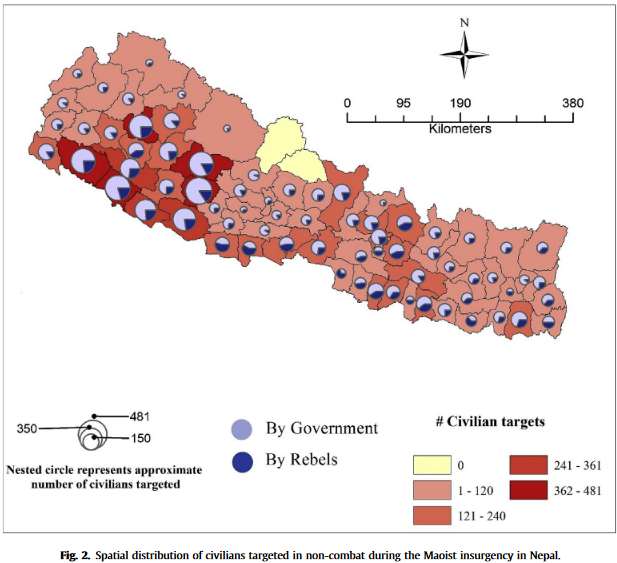
\includegraphics[width=\textwidth,height=\textheight,keepaspectratio]{Nepalkillings.png}
	\end{figure}
\end{frame}

\begin{frame} 
	\frametitle{\LARGE{Civilians and Civil War}}
	\begin{itemize}
		\item This conflict illustrates that civilian targeting was committed by both sides throughout the conflict. \pause
		\item This means it was a systemic feature of the conflict. \pause
		\item Civil wars, arguably more than other kinds of war, can incentivize civilian victimization. Why? \pause
		\item \textbf{The civilian population is inextricably linked to the conflict.}
	\end{itemize}
\end{frame}

\begin{frame} 
	\frametitle{\LARGE{Civilians and Civil War}}
Civilians, in many ways, are caught between (at least) two competing forces in any civil war.
	\begin{itemize}
		\item Rebels use the civilian population to conceal themselves, which may involve coercion. \pause
		\item Rebels may also draw support from the civilian population, such as food or currency. \pause
		\item Without a supply of foreign fighters, rebels also must recruit from the population. Recruitment may be forced. \pause
		\item Rival rebel groups may demand civilians aid them, creating mutually incompatible demands.
	\end{itemize}
\end{frame}

\begin{frame} 
	\frametitle{\LARGE{Civilians and Civil War}}
Civilians, in many ways, are caught between (at least) two competing forces in any civil war.
	\begin{itemize}
		\item State forces know that the rebels are hiding in the civilian population. \pause
		\item States experiencing civil war tend to have lower state capacity, which impacts the state's ability to gather intelligence on rebel membership. \pause
		\item In most cases, state forces struggle to distinguish between true civilians and rebels, which may lead them to target civilians mistakenly. \pause
		\item State forces may also attempt to collectively punish civilians for their (alleged) support of the rebels.
	\end{itemize}
\end{frame}

\begin{frame} 
	\frametitle{\LARGE{Civilians and Civil War}}
	\begin{itemize}
		\item Violence against civilians can be either \textbf{selective} or \textbf{indiscriminate}, and committed by either or both rebels and government forces. \pause
		\item What motivates where and when this violence occurs?		
	\end{itemize}
\end{frame}

\begin{frame} 
	\frametitle{\LARGE{Logic of Violence}}
Kalyvas' \textit{The Logic of Violence in Civil War} (2006) is a foundational examination of the subject.
	\begin{itemize}
		\item Civil wars create \textbf{fractured sovereignty}: rebels and government forces each control different areas. \pause
		\item Each side faces an \textbf{identification problem}: both the state and the rebels want to find and eliminate informants for the other side that are hiding in their territory (as well as rebels hiding in the population). \pause
		\item In areas held by the rebels, these informants will pass information to the state.
		\item In areas held by the state, these informants will pass information to the rebels. 
	\end{itemize}
\end{frame}

\begin{frame} 
	\frametitle{\LARGE{Logic of Violence}}
	\begin{itemize}
		\item The civilian population, generally, will cooperate with whoever is currently in control of their territory. \pause
		\begin{itemize}
			\item Informants come from the civilian population, but not all civilians are informants. \pause
		\end{itemize}
		\item Territorial control requires a credible armed presence by an actor.
		\item \textbf{Civilian informants will only collaborate with a given side as long as they believe there is a strong likelihood that they will be punished for helping the other side (``defection").}
	\end{itemize}
\end{frame}

\begin{frame} 
	\frametitle{\LARGE{Logic of Violence}}
	\begin{itemize}
		\item Different levels of control of an area impact collaboration and defection. \pause
		\item Higher levels of control lead to higher (lower) levels of collaboration (defection) by the population that lives there. \pause
		\item Generally, this means rebels hold rural areas while state holds urban ones. \pause
		\item \textbf{Different levels of territorial control predict different types of violence.}
	\end{itemize}
\end{frame}

\begin{frame} 
	\frametitle{\LARGE{Logic of Violence}}
	\begin{itemize}
		\item \textbf{Selective violence} is only effective when an actor has the information to target their enemies precisely. \pause
		\item This information comes from civilian informants, who will only provide this information to a side if they believe that side is strong enough to shield them from retaliation. 
		\begin{itemize}
			\item Another way to say this is that they will only denounce side A's supporters when side B convincingly controls their territory. \pause
		\end{itemize}
	\end{itemize}
\end{frame}

\begin{frame} 
	\frametitle{\LARGE{Logic of Violence}}
	\begin{itemize}
		\item \textbf{Indiscriminate violence} is most effective when used against populations that support the opposing side. \pause
		\item Why ever use indiscriminate violence? If actors lack information to precisely target their violence against supporters of the opposing side (selective violence), they instead attack populations in which they suspect those supporters are hiding. 
	\end{itemize}
\end{frame}


\begin{frame} 
	\frametitle{\LARGE{Logic of Violence}}
	\begin{itemize}
		\item \textbf{Selective violence} is expected in those areas where a side has dominant but not complete control, as information from denunciation enables direct targeting of supporters of the opposing side. \pause
		\item \textbf{Indiscriminate violence} is expected in the areas in which an organization has no foothold, as it is unlikely to harm its own supporters.
		\item The least amount of violence will occur where both sides have equal power, as neither will be able to shield their informants from retaliation, so no selective violence will occur due to lack of information, while indiscriminate violence would harm their own supporters.
	\end{itemize}
\end{frame}

\begin{frame} 
	\frametitle{\LARGE{Logic of Violence Wrap-Up}}
Kalyvas' model is foundational, but subsequent research has expanded on it.
	\begin{itemize}
		\item Rebel groups may rationally consider the impact of indiscriminate violence on both domestic and international support. \pause
		\item Rebel groups may be less likely to victimize civilians if they are especially dependent on local resources. \pause
		\item Not entirely clear that these accounts explain all violence against civilians in civil wars, especially performative or sexual violence.
	\end{itemize}
\end{frame}

\begin{frame} 
	\frametitle{\LARGE{Central Question 2}}
	\centering
	\Large{Does a rebel group's ideology matter?} 
\end{frame}

\begin{frame} 
	\frametitle{\LARGE{Rebels and Ideology}}
What about ideology and identity? Thus far, we've treated all rebel groups as identical in this regard, but what if they are not? \pause
	\begin{itemize}
		\item \textbf{Ideology} here encompasses whatever set of normative frameworks a group uses.
		\begin{itemize}
			\item Religion, political ideology, ethnic or tribal group solidarity, etc. \pause
		\end{itemize}
		\item Some research has argued that ideology type does not really matter. \pause
		\item More recently, scholars have noticed a disproportionately high representation of Islamist groups in cases of religious civil war. \pause
	\end{itemize}
\end{frame}

\begin{frame} 
	\frametitle{\LARGE{Rebels and Ideology}}
	\begin{itemize}
		\item This has been explained by essentially arguing that religion, in general, is a very effective tool for mobilization.\pause
		\item Religion is effective at solving: \pause
		\begin{itemize}
			\item Collective action problems \pause
			\item Principal-agent problems \pause
			\item Commitment problems \pause
			\item Generally securing resources and support for the group \pause
		\end{itemize}
	\item This brings us to today's reading...
	\end{itemize}
\end{frame}

%\begin{frame} 
%	\frametitle{\LARGE{Walter Review}}
%Group yourselves and answer the following:
%	\begin{itemize}
%		\item What was Walter's main point?
%		\item What are the three waves of civil wars?
%		\item What are the puzzling characteristics of the third wave?
%		\item What explains these characteristics?
%	\end{itemize}
%\end{frame}

\begin{frame} 
	\frametitle{\LARGE{Walter 2017 Review}}
Walter provides an overview of civil war trends and how these conflicts have been theorized.
	\begin{enumerate}
		\item \textbf{First wave}: occurred during the Cold War, with civil wars usually breaking along class lines, and substantial superpower funding and support for either or both sides. \pause
		\item \textbf{Second wave}: lasted from the end of the Cold War to 2003. Civil wars here tended to occur along ethnic separatist lines, with lots of negotiated settlements. \pause
		\item \textbf{Third wave}: 2003-present. Characterized by radical Islamist rebels, frequently with transnational aims.
	\end{enumerate}
\end{frame}

\begin{frame} 
	\frametitle{\LARGE{Walter 2017 Review}}
This third wave has some notable characteristics:
	\begin{itemize}
		\item Rebels tended to be radical \textit{compared to the average view of their host societies}. \pause
		\begin{itemize}
			\item Many of these radical Islamist groups arose in cultures that were already quite Islamic (compared to the West), but the puzzling question was why these groups adopted more extreme views. \pause
		\end{itemize}
	\item Transnational aims were also puzzling: given how rarely rebels win outright victory, how could they expect to do something like create a new caliphate out of parts of several existing states?
	\end{itemize}
\end{frame}

\begin{frame} 
	\frametitle{\LARGE{Walter 2017 Review}}
	\begin{itemize}
		\item Walter argues that this third wave is the first to be fought after the establishment of the modern Internet as we know it. \pause
		\item The connections enabled by the Internet (and later, social media) means that rebels can: \pause
		\begin{itemize}
			\item Spread their own propaganda photos and videos
			\item Deny state propaganda
			\item Network with like-minded sympathizers
			\item Recruit and fund via a global support base \pause
		\end{itemize}
	\item ISIS was not the first, but arguably was the most sophisticated.
	\end{itemize}
\end{frame}

\begin{frame} 
	\frametitle{\LARGE{Online Propaganda Examples}}
	\begin{figure}[ht!]
		\centering
		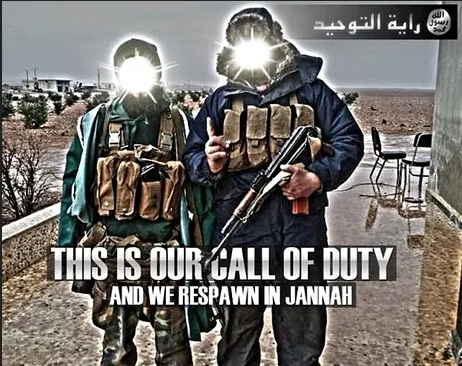
\includegraphics[width=\textwidth,height=0.9\textheight,keepaspectratio]{ISISprop1.png}
	\end{figure}
\end{frame}

\begin{frame} 
	\frametitle{\LARGE{Online Propaganda Examples}}
	\begin{figure}[ht!]
		\centering
		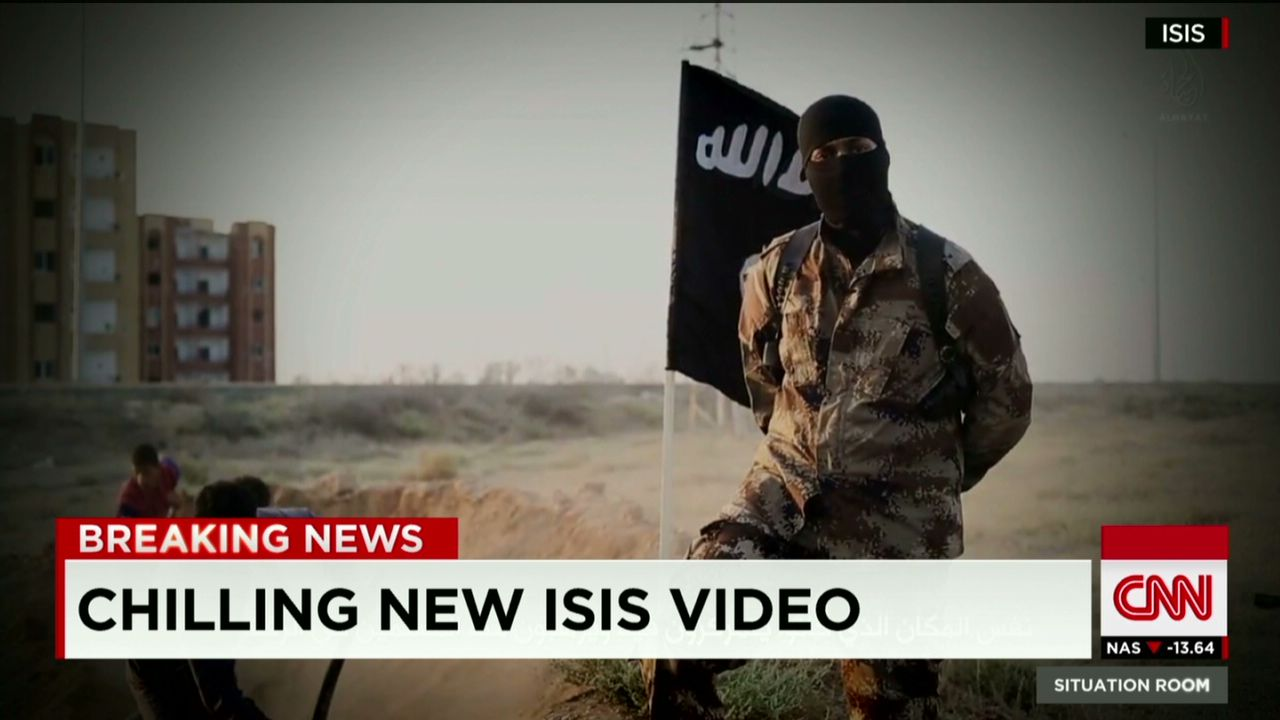
\includegraphics[width=\textwidth,height=0.9\textheight,keepaspectratio]{ISISprop2.jpg}
	\end{figure}
\end{frame}

\begin{frame} 
	\frametitle{\LARGE{Central Question 3}}
	\centering
	\Large{What tactics do rebels use?} 
\end{frame}

\begin{frame} 
	\frametitle{\LARGE{Civil War Tactics: Rebels}}
	\begin{itemize}
		\item Islamic State's swift, massive territorial gains are not typical of most rebel groups.
		\item A majority of civil wars involve \textbf{asymmetric power}, where the state tends to outnumber and outgun the rebels. \pause 
		\item This mean that rebels frequently use a strategy of \textbf{insurgency}, in which small lightly-armed units engage in hit-and-run attacks. \pause 
		\item This strategy does not involve holding (much) territory, making it suited for smaller, weaker groups.  
	\end{itemize}
\end{frame}

\begin{frame} 
	\frametitle{\LARGE{Civil War Tactics: Rebels}}
	\begin{itemize}
		\item The goal of insurgency is to undermine confidence in the state government, and can provoke indiscriminate violence by the state, which increases the rebel recruitment pool. \pause
		\item Rebels blend into a civilian population, making them hard to find. \pause
		\item Endemic commitment problems incentivize rebels to keep fighting even if victory is unlikely.
	\end{itemize}
\end{frame}

\begin{frame} 
	\frametitle{\LARGE{Civil War Tactics: The State}}
	\begin{itemize}
		\item One option for countering insurgency is \textbf{indiscriminate violence} by the state. \pause 
		\item This can occur for multiple reasons: \pause
		\begin{itemize}
			\item State attempts to intimidate civilians into withholding support for rebels via reprisals. \pause
			\item State attempts to remove rebel support by removing civilians. \pause
			\item State lacks information on rebels and its attempts at selective violence actually feel indiscriminate to the population.
		\end{itemize}
	\end{itemize}
\end{frame}

%https://cisac.fsi.stanford.edu/mappingmilitants/profiles/liberation-tigers-tamil-elam#highlight_text_16255
%and wiki
\begin{frame} 
	\frametitle{\LARGE{Sri Lanka and the LTTE}}
	\begin{itemize}
		\item \textbf{Liberation Tigers of Tamil Eelam}: Tamil separatist rebel movement located in northeastern Sri Lanka. \pause
		\item Goal: independent state for Hindu Tamils, located in northeastern Sri Lanka. \pause
		\item Formed in 1972 and carried out its first attack in 1983. \pause
		\item Notable for extensive and skilled use of suicide bombing, as well as their resemblance of a conventional military in their organization.
	\end{itemize}
\end{frame}

%https://en.wikipedia.org/wiki/Sri_Lankan_Civil_War#/media/File:Location_Tamil_Eelam_territorial_claim.png
\begin{frame} 
	\frametitle{\LARGE{LTTE Territory}}
	\begin{figure}[ht!]
		\centering
		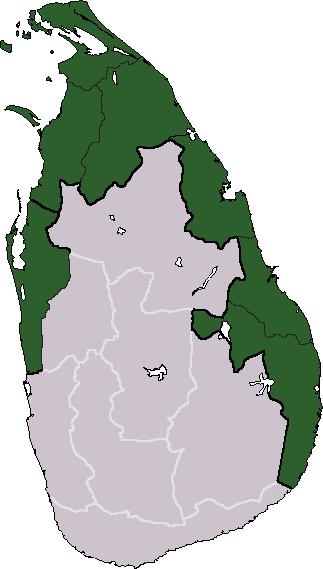
\includegraphics[width=\textwidth,height=0.9\textheight,keepaspectratio]{LTTEterritory.png}
	\end{figure}
\end{frame}

\begin{frame} 
	\frametitle{\LARGE{LTTE Collapse}}
	\begin{itemize}
		\item Despite their multi-decade group survival and skill in insurgency, LTTE was militarily defeated in 2009. \pause
		\item This military victory was possible in part due to a reckless disregard by state forces for civilian lives in LTTE-held provinces. \pause
		\item LTTE was conclusively defeated, but at the cost of massive human rights violations due to indiscriminate violence by the state.
	\end{itemize}
\end{frame}

\begin{frame} 
	\frametitle{\LARGE{Counterinsurgency}}
	\begin{itemize}
		\item Another option is \textbf{counter-insurgency (COIN)}: a ``hearts and minds'' approach that focuses on winning population loyalty through providing security and services, decreasing rebel support. \pause
		\item US and coalition forces in Iraq and Afghanistan turned to COIN in an effort to address the ongoing insurgency. \pause
	\end{itemize}
\end{frame}

\begin{frame} 
	\frametitle{\LARGE{COIN in Iraq}}
	\begin{figure}[ht!]
		\centering
		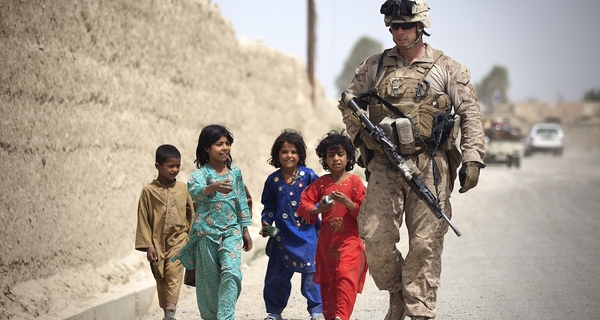
\includegraphics[width=\textwidth,height=\textheight,keepaspectratio]{COIN.jpg}
	\end{figure}
\end{frame}

\begin{frame} 
	\frametitle{\LARGE{COIN in Iraq}}
	\begin{figure}[ht!]
		\centering
		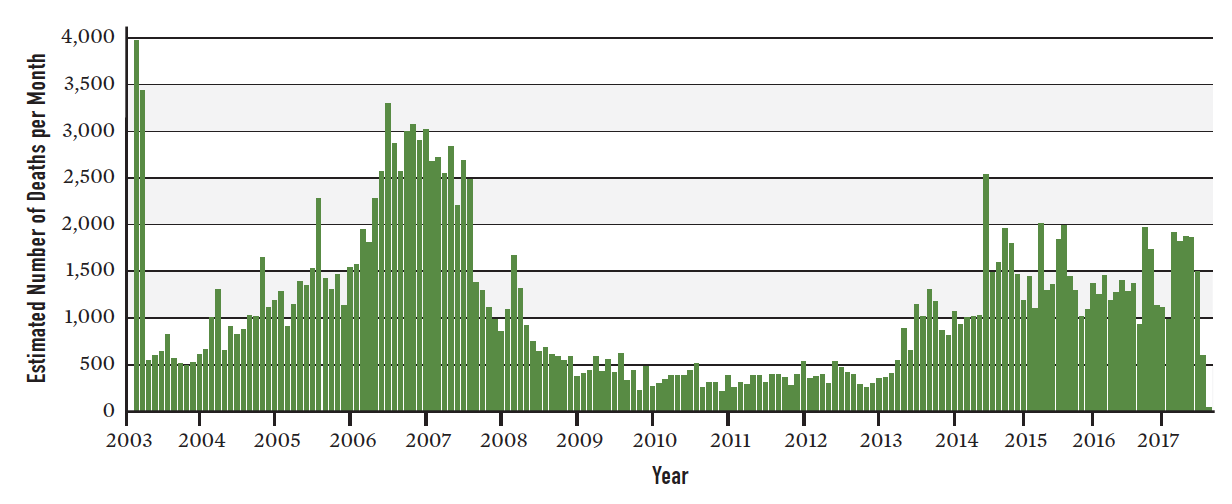
\includegraphics[width=\textwidth,height=\textheight,keepaspectratio]{./surge.png}
	\end{figure}
\end{frame}

\begin{frame} 
	\frametitle{\LARGE{COIN Effectiveness}}
So, did the COIN strategy work? Not really, but...
	\begin{itemize}
		\item COIN required \textbf{massive} amounts of troops and resources - more than US policymakers were often willing to provide. \pause
		\item US troops were hindered by cultural barriers; attempts to address these came too late. \pause
		\item Decreasing domestic US support for these wars prevented the kind of long-term engagement with local populations required to make COIN truly effective. \pause
		\item US state-building failures further compounded these problems.
	\end{itemize}
\end{frame}

\begin{frame} 
	\frametitle{\LARGE{Central Question 4}}
	\centering
	\Large{Why do civil wars last so long?} 
\end{frame}

\begin{frame} 
	\frametitle{\LARGE{Why Do Civil Wars Last So Long?}}
	\begin{figure}[ht!]
		\centering
		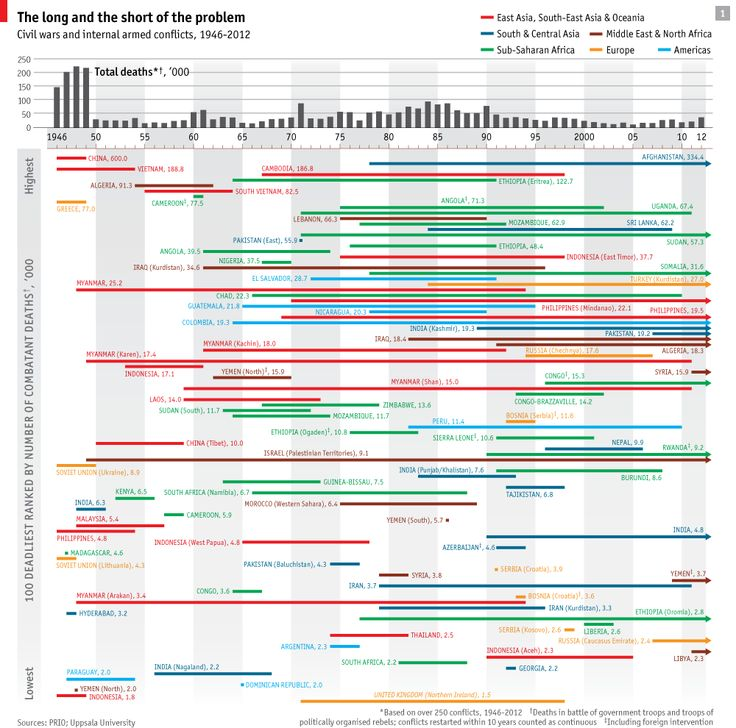
\includegraphics[width=\textwidth,height=0.9\textheight,keepaspectratio]{civil war duration.jpg}
	\end{figure}
\end{frame}

\begin{frame} 
	\frametitle{\LARGE{Why Do Civil Wars Last So Long?}}
	\begin{itemize}
		\item Average civil war lasts 6-7 years, and some last much longer. Why? \pause
		\item Rebels are aware of their weakness compared to the state, and use insurgency tactics to avoid open battles where the state can use its greater strengths. \pause
		\item State may struggle to find rebels, especially with a supportive population. \pause
		\item Disarmament commitment problems incentivize rebels to keep fighting rather than risk being defenseless.
	\end{itemize}
\end{frame}

\begin{frame} 
	\frametitle{\LARGE{How Does a Civil War End?}}
	\begin{itemize}
		\item Historically, most civil wars end in a victory for one side or a negotiated settlement. \pause
		\item If a civil war ended in a victory, \textit{usually} it was a victory for state forces. \pause
		\item Negotiated settlements became more common in the 1990s, likely due to increased UNSC willingness to intervene by providing peacekeeping forces.	
	\end{itemize}
\end{frame}

\begin{frame} 
	\frametitle{\LARGE{How Does a Civil War End?}}
International institutions can help negotiated settlements in a number of ways. \pause 
	\begin{itemize}
		\item Intervention to impose costs on actors using force is tough (peace enforcement). \pause 
		\item However, maintaining peace following the cessation of violence has been possible (peacekeeping). \pause
		\item Peacekeepers can solve commitment problems by monitoring agreeements and warning about renewed aggression. Neutral third parties can provide security for disarmed rebels. \pause
		\item Encouraging development of domestic institutions is the best way to prevent civil conflict in the first place, but is difficult in practice.
	\end{itemize}
\end{frame}

\end{document}
